\setcounter{page}{1}
\section*{Zielsetzung}

Ziel dieses Versuches ist es, sich mit der Funktionsweise eines Reinst-Germanium-Detektors
für die Gamma-Spektroskopie vertraut zu machen. Anschließend wird nach einer Energieeichung
des Detektors, versucht aktive Nuklide zu identifizieren.

\section{Theorie}
\label{sec:Theorie}

Bei der Gamma-Spektroskopie handelt es sich um die Messung von Gammastrahlung (Photonen).
Dringt ein Photon in die Materie eines Absorbers ein, kann es dort eine vielzahl von Wechselwirkungen vollziehen.
Durch diese erfährt es Intensitätsverluste, welche abhängig von der
Schichtdicke $D$, der Anzahl der Elektronen pro Volumeneinheit n und dem Wirkungsquerschnitt $\sigma$ der Photonen sind:
\begin{align}
  N(D) &= \symup{N}_0\,\cdot\,\symup{exp}(-\mu\cdot\sigma)\\
  \mu &= \symup{n}\cdot\sigma\\
\end{align}
Dabei steht $N$ für die Strahlintensität ($\symup{N}_0$ für die Ursprüngliche).
$\mu$ wird als Extinktionskoeffizienten bezeichnet, und ist der reziproke Wert der
mittleren Reichweite $\bar{x}$ der Photonen. Der Wirkungsquerschnitt $\sigma$ ist ein Maß
für die Wahrscheinlichkeit einer Wechselwirkung.

\subsection{Wechselwirkungen}
\label{sec:Wechselwirkungen}

Bei den Wechselwirkungen stehen besonders der \textbf{(innere) Photoeffekt}, der \textbf{Comptoneffekt} und
die \textbf{Paarbildung} im Vordergrund.

Der \textbf{Photoeffekt} tritt auf wenn das Photon mit einem Hüllenelektron (bevorzugt aus
der K-Schale) wechselwirkt. Dabei nimmt das Elektron das Photon auf und wird aus der
Hülle gelöst, wobei das enstehende Loch anschließend unter dem emittieren von Röntgenstrahlung von Elektronen höherer Schalen aufgefüllt wird.
Damit dieser Effekt autreten kann, muss die Photonenergie größer als die Bindungsenergie des Elektrons sein.
Da bei diesem Vorgang das Photon vernichtet wird, und die Röntgenstrahlung selten den Absorber verlassen kann,
wird die gesamte Energie des Teilchens im Absorber deponiert. Der Wirkungsquerschnitt des Photoeffekts ist dabei
abhängig von der Kernladungszahl $Z$, und der Quantenenergie $E$:
\begin{align}
  \sigma_{\symup{Ph}}\,\sim\,Z^{\alpha}\,\cdot\,E^{\delta}\\
\end{align}
Die Faktoren $\alpha$ und $\delta$ sind selber abhängig vom Energiebereich eines Strahlers, und liegen für
natürliche Strahler bei $4 < \alpha < 5$ und $\delta \approx -3.5$.


Der \textbf{Comptoneffekt} ist vergleichbar mit einem unelastischen Stoß zwischen
dem Photon und einem freien ruhenden punktförmigen Elektron. Dabei gibt das Photon
bei der Wechselwirkung einen Teil seiner Energie dem Elektron in Form von kinetischer Energie, und
ändert dabei die Richtung seiner Flugbahn (vergleiche Abb. \ref{fig:compton_skizze}).
\begin{figure}
  \centering
  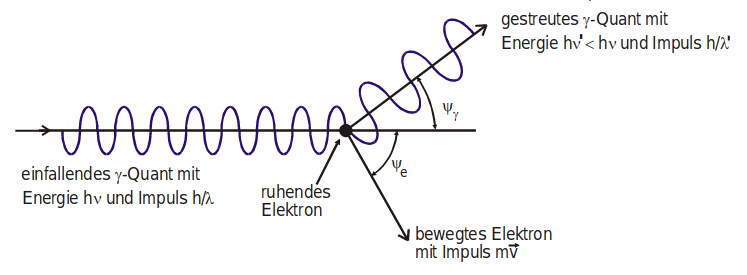
\includegraphics[width=0.8\textwidth]{compton_skizze.png}
  \caption{Darstellung des Comptoneffekts \cite{anleitungv18}.}
  \label{fig:compton_skizze}
\end{figure}
Die Energie des Elektrons ergibt sich zu:
\begin{align}
  E_l &= E_\gamma \,\frac{\varepsilon(1-\symup{cos}\,\Psi_\gamma)}{1+\varepsilon(1-\symup{cos}\,\Psi_\gamma)}\\
  \varepsilon &= E_\gamma\,/\,(\symup{m}_0 \symup{c}^2)\\
\end{align}
Wobei $E_\gamma$ die Photonenergie, $\Psi_\gamma$ den Winkel des gestreuuten Photon,
$\symup{m_0}$ die Ruhemasse des Elektrons und c die Lichtgeschwindigkeit darstellt.
Da das Photon beim Comptoneffekt nie seine gesamte Energie deponiert, ist er ein
eher unerwünschter Effekt bei der Gamma-Spektroskopie. Sein Wirkungsquerschnitt $\sigma_{\symup{Co}}$
fällt mit steigender Photonenergie, und für $\varepsilon\, \to \, 0$ geht er in den
Thomsonschen Streuquerschnitt $\sigma_{\symup{Th}}$ über.

Bei der \textbf{Paarbildung} spaltet sich das Photon in ein Elektron und, dessen Antiteilchen, ein Positron.
Dafür benötigt das Photon eine Energie, die größer ist als die zweifache Ruhemasse des Elektrons.
Da das Photon in seinem eigenen Ruhesystem ruht, braucht es einen Stoßpartner für die Paarbildung.
Aufgrund der auftretenden Rückstoßenergie, die auf den Stoßpartner wirkt, braucht es bei der
Elektron-Elektron Wechselwirkung sogar die vierfache Ruhemasse für den Paarbildungsprozess.
Der Wirkungsquerschnitt $\sigma_{\symup{Pa}}$ der Paarbildung ist abhängig von dem Ort der Wechselwirkung.
Denn je nachdem wo in der Hülle des Atoms die Wechselwirkung stattfindet, erfährt das Photon eine unterschiedlich
starke Abschirmung.

Zur Darstellung der Wirkungsquerschnitte der beschriebenen Wechselwirkungen, ist in Abb. \ref{fig:mu_koeff}
die Energieabhängigkeit der verschiedenen Extinktionskoeffizienten $\mu$ für Germanium abgebildet.
\begin{figure}
  \centering
  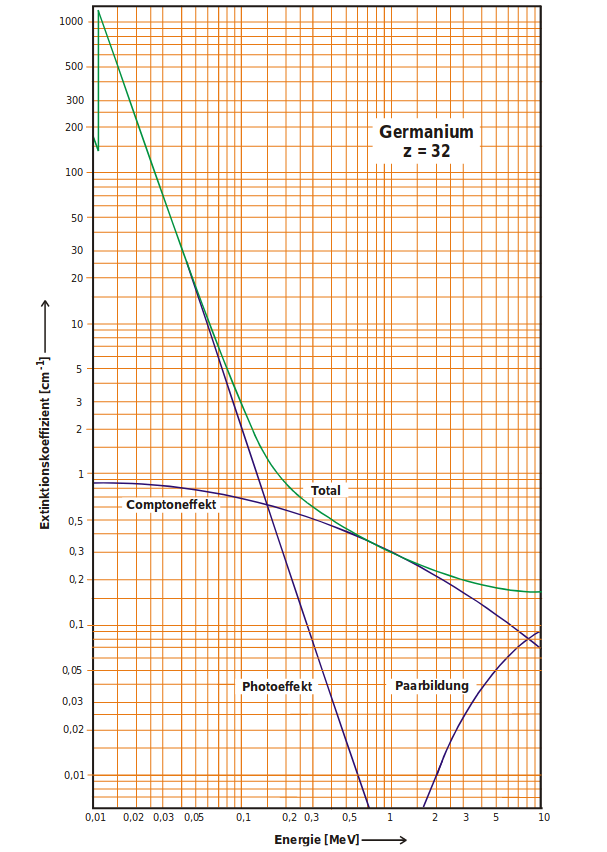
\includegraphics[width=0.95\textwidth]{mu_koeff.png}
  \caption{Extinktionskoeffizienten der verschiedenen Wechselwirkungen für Germanium \cite{anleitungv18}.}
  \label{fig:mu_koeff}
\end{figure}

\subsection{Funktionsweise des Reinst-Germanium-Detektors}

Bei dem Germanium-Detektor handelt es sich um einen \textbf{Halbleiter-Detektor}.
Er besteht im Grunde aus einem \textbf{p-dotierten}- und einem \textbf{n-dotierten}-Bereich, welche
sich durch einen Überschuss an Elektronen bzw. Elektronenlöchern kennzeichnen.
An den Grenzflächen dieser Bereiche rekombinieren die Ladungsträger und bilden eine
verarmte Zone. Diese verarmte Zone wird maximiert, indem eine äußere Spannung angelegt wird, sowie
eine möglichst ungleich verteilte Dotierung gewählt wird. Wenn ein Photon in diese
vergrößerte ($\SI{6}{\centi\meter}$) verarmte Zone eindringt, enstehen mehrere
Paare aus Elektronen und Löchern, welche durch die herschende äußere Spannung an verschiedene
Elektroden gesaugt werden. Dabei muss die Spannung hoch genug sein, um die Ladungsträger zu trennen
bevor sie rekombinieren können. Aus dem enstehenden Ladungsimpuls bei der Trennung, lässt sich
über geeignete Verfahren auf die Energie der Photonen schließen.
Die äußere Spannung darf dabei nicht zu hoch gewählt werden, da durch
thermische Aktivierung stets ein Strom ensteht der, durch die Spannung verstärkt,
sich negativ auf den Detektor auswirkt. Um diesem Strom entgegenzuwirken, wird der
Detektor auf $\SI{77}{\kelvin}$ gekühlt.

Der Reinst-Germanium-Detektor ist zylinderartig aufgebaut, und hat den in Abb. \ref{fig:detektor}
dargestellten Querschnitt. Seinen n-dotierten Bereich bildet die mit Lithium diffundierte Oberfläche,
während seine innere Oberfläche mit Gold diffundiert ist, und den p-dotierten Bereich darstellt.
Um den Detektor herum ist eine Aluminiumschicht zum abfangen von Photonen mit geringer Energie.
Die gesamte Apperatur ist mit Blei umgeben um Strahlung von außerhalb abzuhalten.
Der Detektor kann Photonenenergie von einigen MeV messen.
\begin{figure}
  \centering
  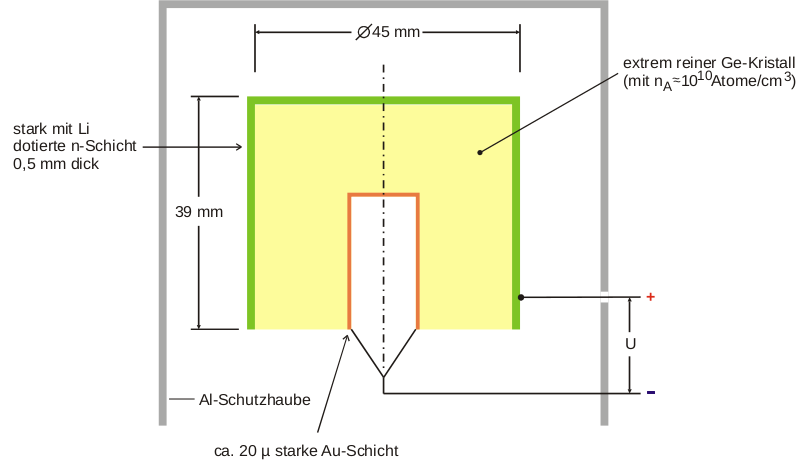
\includegraphics[width=0.95\textwidth]{detektor.png}
  \caption{Querschnitt des Reinst-Germanium-Detektor \cite{anleitungv18}.}
  \label{fig:detektor}
\end{figure}

Als nächstes soll auf das \textbf{energetische Auflösungsvermögen} des Detektors eingegangen
werden. Dieses ist ein Maß dafür, wie genau der Detektor nah aneinander liegende Spektrallinien
voneinander unterscheiden kann. Dafür wird eine Halbwertsbreite $\Delta E_{1/2}$ eingeführt, auf dessen
Ursprung später noch eingegangen wird. Aus der Betrachtung der Ladungsträgererzeugung als
Poisson-verteilter Prozess, lässt sich die Halbwertsbreite wie folgt beschreiben:
\begin{align}
  \Delta E_{1/2} \approx 2.35\cdot(0.1\,E_\gamma\,E_{\symup{El}})^{\frac{1}{2}}
\end{align}
Dabei steht $E_{\symup{El}}$ für die Bildungsenergie eines Paares von Elektron und Loch.
Für einen Germanium-Detektor liegt die typische Halbwertsbreite bei
$\Delta E_{1/2} =\SI{895}{\electronvolt}$.
Problematisch für das energetische Auflösungsvermögen sind jedoch Effekte wie das Rauschen
des Verstärkers, die Feldinhomogenität durch die Ladungsträger sowie der zuvor genannte
Strom durch die thermische Aktivierung und der äußeren Spannung.
Diesen wird Abhilfe geschaffen, indem nicht nur der Detektor sondern auch der
angeschlossene Verstärker gekühlt wird. Da die Feldinhomogenität durch eine hohe
äußere Spannung verringert werden kann (welche den störenden Strom erhöht), muss ein Mittelmaß
für diese gefunden werden.

Zuletzt wird noch auf die \textbf{Effizienz} des Detektors eingegangen.
Diese steht für die Energieabhängigkeit der Wahrscheinlichkeit für die vollständige Absorption
eines Photons, da diese zum großen Teil ihre Energie nicht komplett im Detektor deponieren.
Dies folgt daraus dass für eine vollständige Deponierung nur der Photoeffekt fähig ist.
